%==============================================================================
% Sjabloon onderzoeksvoorstel bachelorproef
%==============================================================================%
% Compileren in TeXstudio:
%
% - Zorg dat Biber de bibliografie compileert (en niet Biblatex)
%   Options > Configure > Build > Default Bibliography Tool: "txs:///biber"
% - F5 om te compileren en het resultaat te bekijken.
% - Als de bibliografie niet zichtbaar is, probeer dan F5 - F8 - F5
%   Met F8 compileer je de bibliografie apart.
%
% Als je JabRef gebruikt voor het bijhouden van de bibliografie, zorg dan
% dat je in ``biblatex''-modus opslaat: File > Switch to BibLaTeX mode.

\documentclass{hogent-article}

\usepackage{lipsum} % Voor vultekst

%------------------------------------------------------------------------------
% Metadata over het artikel
%------------------------------------------------------------------------------

%---------- Titel & auteur ----------------------------------------------------

% TODO: (fase 2) geef werktitel van je eigen voorstel op
\PaperTitle{Op welk punt in de groei van een organisatie is het implementeren van een ERP-systeem van nut?}
% Dit is typisch de opdracht en het vak waarvoor dit artikel geschreven is, bv.
% ``Verslag onderzoeksproject Onderzoekstechnieken 2018-2019''
\PaperType{Paper Research Methods: onderzoeksvoorstel}

% TODO: (fase 1) vul je eigen naam in als auteur, geef ook je emailadres mee!
\Authors{Sebastiaan Cuypers\textsuperscript{1}} % Authors

% Als het hier effectief gaat om een voorstel voor de bachelorproef, dan ben je
% hier verplicht de naam van je co-promotor in te vullen. Zoniet, dan kan je het
% leeg laten.
\CoPromotor{}



% Contactinfo: Geef hier de contactgegevens van elke auteur van het artikel (en
% indien van toepassing ook van de co-promotor).
\affiliation{
  \textsuperscript{1} \href{mailto:sebastiaan.cuypers@student.hogent.be}{sebastiaan.cuypers@student.hogent.be}
}


%---------- Abstract ----------------------------------------------------------

\Abstract{% TODO: (fase 6)
De overstap voor een organisatie naar het in gebruik nemen van een ERP-systeem komt met een heel deel vragen waarvan de antwoorden volledig afhangen van de organisatie zelf. Dit houdt in de grootte, sector, budget en know-how van de organisatie. Door middel van bedrijfs profielen zullen verschillende  ERP-systemen vergeleken worden en zo de beste keuzes per profiel geselecteerd worden.
}

%---------- Onderzoeksdomein en sleutelwoorden --------------------------------
% TODO: (fase 2) Vul de sleutelwoorden aan.

% Het eerste sleutelwoord beschrijft het onderzoeksdomein. Je kan kiezen uit
% deze lijst:
%
% - Mobiele applicatieontwikkeling
% - Webapplicatieontwikkeling
% - Applicatieontwikkeling (andere)
% - Systeembeheer
% - Netwerkbeheer
% - Mainframe
% - E-business
% - Databanken en big data
% - Machineleertechnieken en kunstmatige intelligentie
% - Andere (specifieer)
%
% De andere sleutelwoorden zijn vrij te kiezen.

\Keywords{Onderzoeksdomein; E-business; ERP; Groei}
\newcommand{\keywordname}{Sleutelwoorden} % Defines the keywords heading name

%---------- Titel, inhoud -----------------------------------------------------

\begin{document}

\flushbottom % Makes all text pages the same height
\maketitle % Print the title and abstract box
\tableofcontents % Print the contents section
\thispagestyle{empty} % Removes page numbering from the first page


%------------------------------------------------------------------------------
% Hoofdtekst
%------------------------------------------------------------------------------

\section{Inleiding}

% TODO: (fase 2) introduceer je gekozen onderwerp, formuleer de onderzoeksvraag en deelvragen. Wat is de doelstelling (is die S.M.A.R.T.?), wat zal het resultaat zijn van het onderzoek (een Proof-of-Concept, een prototype, een advies, ...)? Waarom is het nuttig om dit onderwerp te onderzoeken?

Dit onderzoek zou een groeiende organisatie moeten helpen bij het maken van de beslissing om een ERP-systeem al dan niet te implementeren. En zal antwoorden bevoorraden op de vragen die zich voordoen bij het begin van de implementatie van zo'n systeem. Directe kosten en kosten op langere termijn alsook de verschillende mogelijkheden waarop het systeem op de meest toepasselijke manier kan uitgerold worden voor een organisatie. En ook of de organisatie in kwestie al dan niet geschikt is voor de implementatie van een ERP-systeem.

\section{Overzicht literatuur}

% TODO: (fase 4) schrijf de literatuurstudie uit en gebruik waar gepast referenties naar de vakliteratuur.

% Refereren naar de literatuur kan met:
% \autocite{BIBTEXKEY} -> (Auteur, jaartal)
% \textcite{BIBTEXKEY} -> Auteur (jaartal)

ERP en een acroniem die staat voor Enterprise Resource Planning. Dit is een software pakket die het mogelijk maakt om business processen van een organisatie te automatiseren en onderling te laten communiceren om zo een de efficiëntie van de organisatie te verhogen. De meest voorkomende processen die in aanmerking komen zijn Customer Relationship Management (CRM), Human Resource Management (HRM), Supply Chain Management, productie... \autocite{Microsoft2022}



\begin{figure}[h!]
    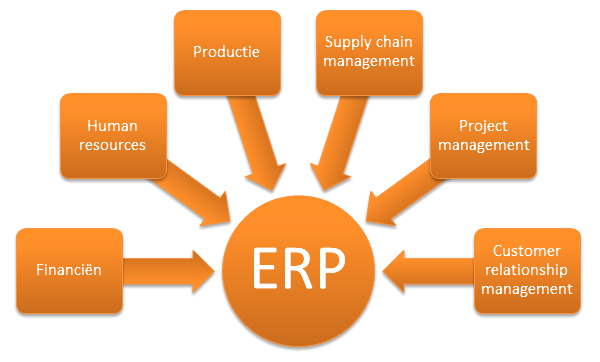
\includegraphics[width=8.5cm]{img/processen.png}
    \caption{ERP-processen (implementatie-erp.nl)}
\end{figure}


\subsection{Processen van ERP}
Wanneer een organisatie een ERP systeem wil implementeren kan die ervoor kiezen om maar enkele processen op te nemen in het systeem. We zullen beginnen met een beknopte beschrijving van deze processen. \par

Custummor Relationship Management (CRM) staat in voor de relaties met klanten te onderhouden. Deze zorgt ervoor dat de klanttevredenheid en loyaliteit hoog gehouden wordt. Dit wordt mogelijk gemaakt door verscheidene subprocessen waarvan het identifecerren van kansen en het creëren van klantenkennis. \autocite{Rababah2011} \par

Human Resource Management (HRM) omvat alles wat te maken heeft met interne zaken met betrekking tot het personeel. Het uiteindelijke doel van HRM is om de beschikbare "resources" zodanig te beheren om de organisatie zo efficiënt mogelijk te laten werken. \autocite{Greenwood2002} \par

Supply Chain Management (SCM) zorgt ervoor dat alle verschuivingen van goederen, financiële middelen en materialen vlot verloopt waardoor deze middelen geraken waar ze nodig zijn. \autocite{Oracle2022} \par

Productie heeft als taak het beheren van het productieproces. Door dit systeem kan ieder onderdeel van een product getraceerd worden aan de hand van lotnummers waardoor veel onderdelen van het productieproces geautomatiseerd kunnen worden. Bijvoorbeeld als onderdeel A uit stock gehaald wordt wordt dit doorgegeven aan de supply chain zodat onderdeel A automatisch kan worden bijbesteld indien nodig. \autocite{Captivea2022} \par

Financial management volgt alle financiële transacties van een organisatie op en voert deze ook uit. Deze module wordt ook gebruikt voor risico 's van bepaalde transacties in te schatten. Alsook tal van andere taken in verband met belastingen en openstaande schulden en lasten. Dit systeem geeft ook verslag uit over de financiële status van de organisatie. \autocite{Ding2015} \par

Als laatste zorgt Project management ervoor dat projectdoelstellingen gehaald worden en deze doelstellingen ook voldoen aan de gestelde criteria. Dit wordt behaald door middel van verschillende processen, vaardigheden, kennis en ervaring samen te doen werken om zo de doelstelling te bereiken. \autocite{Schwalbe2015} \par

Bovenstaande processen zijn de meest voorkomende die organisaties implementeren in hun gang van zaken.

\subsection{Waarom ERP?}

Het grote voordeel aan het gebruik van een ERP-systeem voor een organisatie is dat alle of enkele bijdrijfsprocessen geautomatiseerd worden en zo één groot bedrijfsproces wordt. Hierdoor gaat de efficiëntie van de organisatie omhoog. Door alles één geheel te maken is de kans op menselijke fouten ook sterk gedaald. Dit komt omdat de data van een programma die bijvoorbeeld die voorraad bijhoudt niet meer manueel ingevoerd moet worden in een ander systeem die verantwoordelijk is voor het maken van orders. Dit gebeurd nu allemaal volautomatisch. \autocite{Schwarz2020} \par

Wat vaak een afknapper is voor organisaties om een ERP-systeem te integreren is de kost van zo 'n systeem. Deze kunnen inderdaad oplopen door licenties en de kosten die de implantatie zelf met zich meebrengt, merk op dat tijdens de implementatie periode het systeem uiteraard nog niet in gebruik genomen kan worden. Een andere reden waardoor een organisatie afgeschrikt kan worden is de initiële complexiteit en de verandering van de interne verandering van de organisatie. Het motto "If it ain't broke, don't fix it" komt iedereen wel bekend voor. Maar als een organisatie deze mentaliteit aanneemt schiet deze organisatie zichzelf in de voet door hun eigen groei in de weg te staan. \autocite{Schwarz2020}\par




\subsection{ERP pakketen}

Vooraleer de implementatie van start kan gaan moet er natuurlijk een ERP-pakket uitgekozen worden. Er bestaan verschillende pakketten, de ene bekender dan de andere, die ook nog een verschillende types van hun product aanbieden die aan verschillende use-cases aaansluiten. In dit onderzoek zullen volgende pakketen gebruikt worden in de vergelijking.\par

\subsubsection{SAP}
SAP ECC staat voor SAP ERP Central Component. En is één van de legacy applicaties van SAP. Het is ontwikkeld op te kunnen samen werken met databanken van derden. ECC is het kernproduct van SAP en is dus ook het meeste gebruikte bij hun klanten. Merk wel op dat SAP ECC een core component is. Dit wil zeggen dat functionaliteiten extra kunnen aangekocht worden naar gelang de noden van de organisatie of zelf nog te ontwikkelen. De ondersteuning van dit pakket zal stoppen in 2027 met andere woorden SAP ECC is niet meer interessant om aan te schaffen. Organisaties die huidig een ECC applicatie draaiende hebben moeten tegen 2027 overschakelen naar SAP S/4HANA.\par

SAP S/4HANA is een geïntegreerd ERP-systeem waar de data in een in-memorydatabase (SAP HANA) opgeslaan wordt. Door de database te integreren kunnen transacties efficiënter uitgevoerd worden en waardoor de prestaties van het systeem stijgen. Een voordeel van S/4HANA is dat het multiplatform is.  Dit wil zeggen dat bepaalde services on-premise gehost kunnen worden en anderen in de cloud. Hierdoor kunnen bedrijfskosten gedrukt worden. \autocite{Syntax2020} \par

SAP Business One is een volledig nieuw systeem ontwikkeld door SAP voor kleinere organisaties waar alle functionaliteiten die een organisatie nodig heeft al ingebouwd heeft. B1 bestaat slechts uit één server waar ECC / S/4HANA uit meerdere bestaan en dus meer data aan kunnen. \autocite{firebearstudio.com2021}\par

\subsubsection{Microsoft Dynamics}

Microsoft Dynamics SL is een ERP-systeem die on-premise gehost wordt bij een organisatie. Dit systeem is gespecialiseerd in projectgestuurde middelgrote organisaties. Het kan namelijk projecten binnen de divisies en locaties van de organisatie automatismen en stroomlijnen. \autocite{Journyx2014}\par

Microsoft Dynamics GP wordt gebruikt voor bedrijfsboekhouding en is de perfecte oplossing voor organisaties die snel groeien. Er is een focus op eenvoud waardoor er vaak modules van derden worden toegevoegd. GP wordt nog tot 2028 ondersteund is dus ook niet meer interessant om in te investeren.\autocite{Journyx2014}\par

Microsoft Dynamics AX is specifiek gericht op de enterprise-sector en is een meertalig ERP-systeem met meerdere valuta. Dit maakt AX de meest complete en configureerbare versie van Dynamics out-of-the-box, perfect voor een brede scope aan industrieën.\autocite{Journyx2014}\par

Microsoft Dynamics NAV is gericht op bedrijven in de productie-, retail-, distributie- en professionele dienstverleningsmarkt. Wat het onderscheidt, is het gemak waarmee het kan worden aangepast voor nichegebruik. Dit maakt het ideaal voor startups en niche bedrijven waarvan de eisen zo snel veranderen dat geen enkel ander kant-en-klaar pakket zal werken. \autocite{Journyx2014}\par

Dynamics 365 Finance & Operations is een ERP-systeem die gebaseerd is in the cloud waardoor dit systeem geschikt is vor grote organisaties. In werkelijkheid bestaat deze enkele implementatie uit twee software liscencies namelijk Dynamics 365 Finance waar de focus ligt op financiën en boekhouding en dynamics 365 Supply chain Management waar de nadruk ligt productie, opslag en distributie.\par

\subsubsection{Infor}
Infor M3 is een systeem die in the cloud gehost wordt en dient voor productie en distributie. Het platform voorziet een krachtige analyse van data waar meerdere bedrijven op meerdere locaties gebruik van kunnen maken. \autocite{Infor2022}\par

\section{Methodologie}

% TODO: (fase 5) beschrijf in detail in welke fasen je onderzoek uiteenvalt, hoe lang elke fase duurt en wat het concrete resultaat van elke fase is. Welke onderzoekstechniek ga je toepassen om elk van je onderzoeksvragen te beantwoorden? Gebruik je hiervoor experimenten, vragenlijsten, simulaties? Je beschrijft ook al welke tools je denkt hiervoor te gebruiken of te ontwikkelen.

Het onderzoek zou als volgt verlopen. Als eerst zullen er bedrijfs profielen opgesteld worden. Hierdoor kan een organisatie zich beter plaatsen in de resultaten die gehaald zullen worden. De profielen zullen gemaakt worden op basis van de grote van het bedrijf in termen van het aantal werknemers en de omzet die de organisatie heeft, de sector waar die zich in bevindt en het budget die de organisatie over heeft voor de implementatie van het systeem. \par

Profiel A zou bijvoorbeeld kunnen staan voor een bedrijf in de marketing sector van met een personeelsaantal van 250+ werknemers. Dit profiel zou dus geen nood hebben aan een module om de productie te beheren aangezien er niets geproduceerd wordt.\par 

Na het opstellen van enkele profielen zullen er verschillende bedrijven gecontacteerd worden die een van bovenstaande pakketten of een ander pakketten distribueren met de vraag om per profiel een offerte te kunnen leveren voor hun oplossing voor de noden van het profiel.\par

Op basis van deze informatie zal er gekeken worden welke oplossing het meest voordelig is voor ieder profiel. Hier wordt er gekeken naar de kost, ondersteuning, schaalbaarheid naar de toekomst en of het platform open staat voor nieuwe technologieën (denk IoT etc.). 

\section{Verwachte conclusies}

% TODO: (fase 6) beschrijf wat je verwacht uit je onderzoek en waarom (bv. volgens je literatuuronderzoek is softwarepakket A het meest gebruikte en denk je dat het voor deze casus ook het meest geschikt zal zijn). Natuurlijk kan je niet in de toekomst kijken en mag je geen alternatieve mogelijkheden uitsluiten. In de praktijk gebeurt het ook vaak dat een onderzoek tot verrassende resultaten leidt, dat maakt het proces nog interessanter!

Voor kleine organisatie zal een pakket zoals SAP Business One waarschijnlijk het voordeligst zijn. Een licentie voor B1 gaan maximum tot 1500 euro voor een pakket waar alle basis benodigdheden al in verwerkt zitten.\par

Vanaf we te maken hebben met een niche sector of een middelmatig tot groot bedrijf is het direct al veel moeilijker om een voorspelling te doen. Hiertoe dienen ook de bovenstaande profielen om organisaties in grote lijnen te kunnen categoriseren en zo voor die bepaalde categorieën en antwoord te bekomen.

%------------------------------------------------------------------------------
% Referentielijst
%------------------------------------------------------------------------------
% TODO: (fase 4) de gerefereerde werken moeten in BibTeX-bestand
% bibliografie.bib voorkomen. Gebruik JabRef om je bibliografie bij te
% houden.

\phantomsection
\printbibliography[heading=bibintoc]

\end{document}
